\let\negmedspace\undefined
\let\negthickspace\undefined
\documentclass[journal]{IEEEtran}
\usepackage[a5paper, margin=10mm, onecolumn]{geometry}
%\usepackage{lmodern} % Ensure lmodern is loaded for pdflatex
\usepackage{tfrupee} % Include tfrupee package

\setlength{\headheight}{1cm} % Set the height of the header box
\setlength{\headsep}{0mm}     % Set the distance between the header box and the top of the text

\usepackage{gvv-book}
\usepackage{gvv}
\usepackage{cite}
\usepackage{amsmath,amssymb,amsfonts,amsthm,mathtools}
\usepackage{algorithmic}
\usepackage{graphicx}
\usepackage{textcomp}
\usepackage{xcolor}
\usepackage{txfonts}
\usepackage{listings}
\usepackage{enumitem}
\usepackage{mathtools}
\usepackage{gensymb}
\usepackage{comment}
\usepackage[breaklinks=true]{hyperref}
\usepackage{tkz-euclide} 
\usepackage{listings}
\def\inputGnumericTable{}                                 
\usepackage[latin1]{inputenc}                                
\usepackage{color}                                            
\usepackage{array}                                            
\usepackage{longtable}                                       
\usepackage{calc}                                             
\usepackage{multirow}                                         
\usepackage{hhline}                                           
\usepackage{ifthen}                                           
\usepackage{lscape}
\begin{document}

\bibliographystyle{IEEEtran}
\vspace{3cm}

\title{1.3.4}
\author{EE24BTECH11002 - Agamjot Singh
}
% \maketitle
% \newpage
% \bigskip
{\let\newpage\relax\maketitle}

\renewcommand{\thefigure}{\theenumi}
\renewcommand{\thetable}{\theenumi}
\setlength{\intextsep}{10pt} % Space between text and floats

\textbf{Question:}
\newline
Find a relation between $x$ and $y$ if the points $\brak{x, y}$, $\brak{1, 2}$ and $\brak{7, 0}$ are collinear. 
\newline
\textbf{Solution:}
\newline
Let the points be $\vec{A}\brak{1, 2} \text{,} \vec{B}\brak{7, 0} \text{ and } \vec{C}\brak{x, y}$.

The collinearity matrix is given by
\begin{align}
	\myvec{\vec{B} - \vec{A} & \vec{C} - \vec{A}}^\top = \myvec{6 & x - 2\\ -2 & y - 2}\\ 
													   \xrightarrow{R_2 = R_2 + 3R_1} \myvec{6 & x - 2\\0 & 3x + y - 8}
\end{align}

For the points to be collinear, the rank of this matrix has to be one.

\begin{align}
	3x + y - 8 = 0
\end{align}

The relation between $x$ and $y$ is a line.

\begin{figure}[h!]
   \centering
   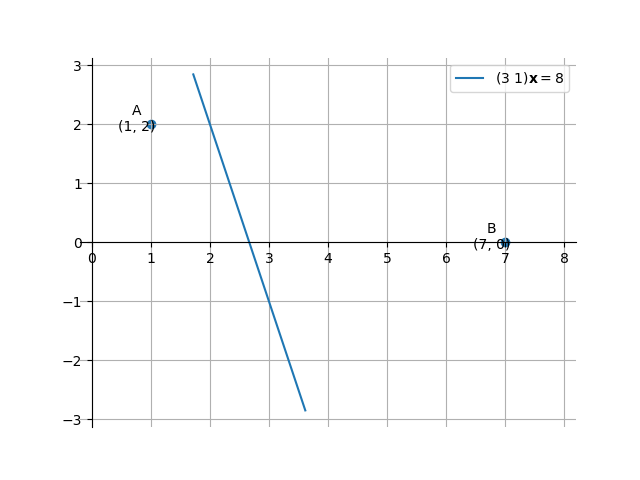
\includegraphics[width=0.7\linewidth]{figs/graph.png}
   \caption{Line which represents the relation between x and y}
\end{figure}

\end{document}
